\begin{figure}
    \begin{center}
    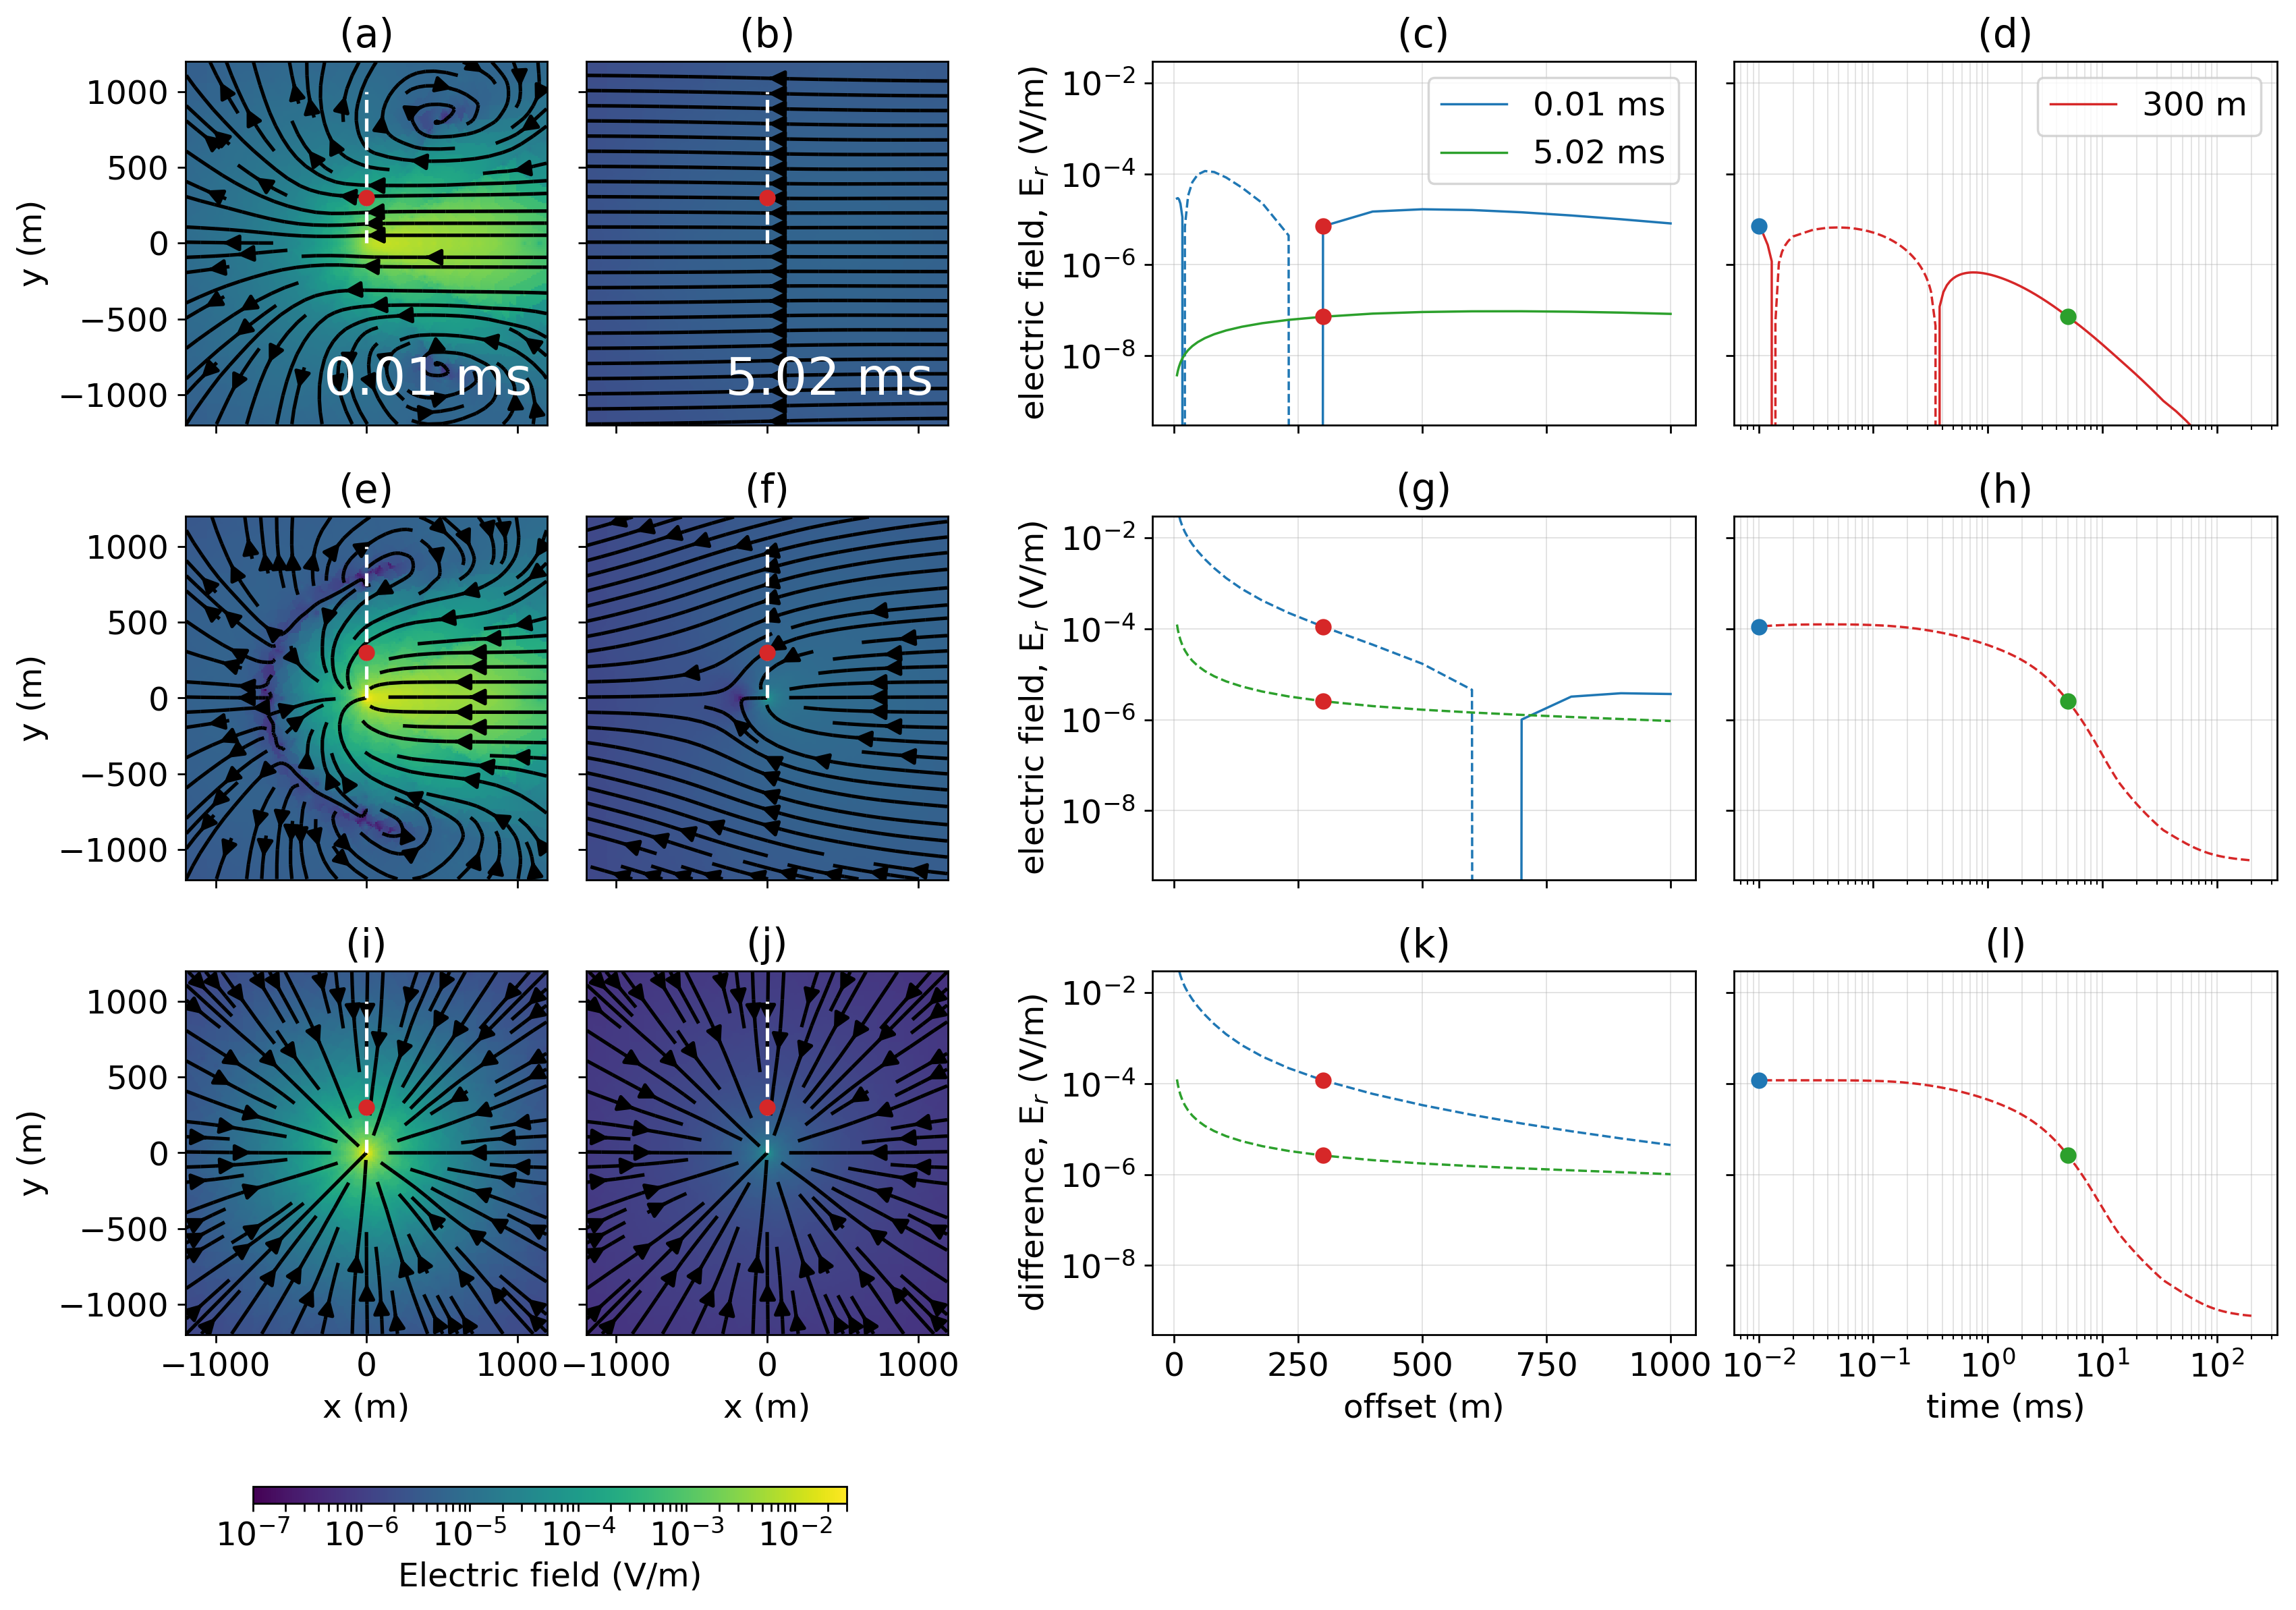
\includegraphics[width=\textwidth]{figures/em_casing/surface_e_fields_overview.png}
    \end{center}
\caption{
    Simulated electric field at the surface of the earth at (a) 0.01ms and (b) 5ms after shut-off for the halfspace model.
    (c) Radial electric field data measured along the survey line shown in white in (a) and (b) at 0.01ms (blue) and 5ms (green).
    (d) Radial electric field as a function of time at 300m along the survey line (shown in the red dot in (a)).
    The red dots in (c) correspond to the data observed at 300m offset
    and the blue and green dots in (d) correspond to the 0.01ms and 5ms data.
    Similar information is shown in (e), (f), (g) and (h) for the model with the conductive casing.
    The difference in the radial electric field data (casing minus halfspace) is shown in (i), (j), (k) and (l).
    %The difference is also shown as a percentage of the halfspace solution at 0.01ms and 5ms in (m)
    %and through time at 300m offset in (n).
}
\label{fig:surface_e_fields_overview}
\end{figure}



